

\documentclass[letterpaper, 10 pt, conference]{ieeeconf} 
\usepackage{graphicx}
\IEEEoverridecommandlockouts                           
\overrideIEEEmargins
\usepackage{booktabs}
\usepackage[table,xcdraw]{xcolor}
\usepackage{svg}
\usepackage{atbegshi}%
\renewcommand*{\thefootnote}{\fnsymbol{footnote}}http://ctan.org/pkg/atbegshi
\AtBeginDocument{\AtBeginShipoutNext{\AtBeginShipoutDiscard}}


\begin{document}
\title{\LARGE \bf
Measurement Based Study of K-V Storage Software*
}

\author{ \parbox{3 in}{\centering Clara Nguyen
        \\
        Electrical Engineering and Computer Science Department\\
         University of Tennessee\\
         {\tt\small ssmit285@vols.utk.edu}}
         \hspace*{ 0.5 in}
         \parbox{3 in}{ \centering Rachel Offutt
        \\
       Electrical Engineering and Computer Science Department\\
         University of Tennessee\\
         {\tt\small roffutt@vols.utk.edu}}
}
\thanks {\textbf{*As a note, this study was created, designed, and carried through for the purpose of course credit for the University of Tennessee's COSC560 course. This study is not made to be publishable research by any means.}}







\maketitle
\thispagestyle{empty}
\pagestyle{empty}


\begin{abstract}

This document aims to analyze and compare different performance metrics of different key-value storage software on both solid state drives and physical drives using both command line arguments and Node.js to run the various tests.

\end{abstract}

\section{INTRODUCTION}

With the rise of the digital age, more and more of society's records are stored digitally to improve ease of access and length of preservation compared to that of paper filing. Storing vast amounts of data digitally means that there needs to be a way not only to store this data efficiently, but also having a way to easily query the data and retrieve the desired data from storage. This is where the creation of databases comes in, a means to store and query large amount of digital data.

\subsection{Databases}
A database can be defined as a collection of data (regardless of size) that is organized in order to be easily accessed, edited, and updated. The data is typically stored in rows and columns, making up various tables, and then indexed in order to find relevant information. When new information is added to the database, the subsequent data may be modified, new data may be added, or obsolete data may be deleted. Workloads are processed by databases so that they may create and update themselves, querying from the contained data within the database and running various applications against it. Computer databases are typically used to contain aggregations of data records or files, such as sales transactions, product catalogs and inventories, and customer profiles (things that can be hashed for easy access to find again).

\subsection{Key-Value Databases}

A key-value database is a type of nonrelational database that uses a simple key-value method to store data. A nonrelational database does not use the tabular schema of rows and columns found in most traditional database systems. Instead, nonrelational databases use a storage model that is optimized for the specific requirements of the type of data being store. A key-value database stores data as a collection of key-value pairs in which a key serves as a unique identifier that will then be searched for in order to find the value. Both keys and values can be anything, ranging from simple objects to complex compound objects. Key-value databases are highly partitionable and allow horizontal scaling at scales that other types of databases cannot achieve. 

In this study, two popular key-value databases, SQL and Redis, are compared in performance on solid state drives (SSD) and hard disk drives (HDD), as well as being run with command line arguments and Node.js.

\section{BACKGROUND}

In this section, the backgrounds and structures of the two software we run our tests on are examined. The first to be covered is SQL Database software, and the second is Redis. 
\subsection{SQL (Structured Query Language)} 
First appearing in 1974 and designed by Donald D. Chamberlin and Raymond F. Boyce, SQL is a domain-specific language programming and designed to help manage data held in databases or for stream processing in a relational data stream management system (RDSMS)[3]. SQL was one of the first commercial languages used for relational modeling by Edgar F. Codd's 1970 paper "A Relational Model of Data for Large Shared Data Banks." However, it is important to note that SQL did not completely adhere to the relational model described by Codd in his paper. Regardless, SQL has become one of the most widely used database languages. SQL excels at handling data where relations between the different variables/data are present. Differing form the older systems before its time, such as the read/write APIs like ISAM (indexed sequential access method) and VSAM (virtual storage access method), SQL boasts two main advantages. Firstly, SQL was the first to introduce the concept of accessing many records with a singular command[4]. The second major improvement is that SQL does not require the need to specify a method of reaching a certain record, for example, the use of an index or not.


SQL was originally designed with relational and tuple relational calculus and consisting of many different kinds of statements, often referred to as sub-languages. Several of these sub-languages are[4]:  
\begin{itemize}
    \item a data query language (DQL)
    \item a data definition language (DDL)
    \item a data control language (DCL)
    \item a data manipulation language (DML)
\end{itemize}


In 1986, SQL became a standard of the American National Standards Institute (ANSI), and in 1987, became a standard of International Organization for Standardization (ISO)[2]. Even after being considered a standard, the standard has been revised to include a wider set of features. The scope of SQL includes data query, data manipulation (insert, update and delete), data definition (schema creation and modification), and data access control. Although SQL is often described as, and to a great extent is, a declarative language, it also includes procedural elements. Despite the existence of such standards, most SQL code is not completely portable among different database systems without adjustments.


SQL has come to adapt and evolve in several ways away from its theoretical foundation of the base relational model and tuple calculus that it was originally designed with. Originally, a table would consist of a set of tuples, while in the current SQL, tables and queries are comprised of lists of rows; the same row also has the ability to appear multiple times, while the order of the rows are use din queries[3].


Despite being one of the most widely used database languages, SQL is not without its critics. There are those who feel that SQL should be completely replaced with a language that adheres more to its original foundation, which SQL has deviated from. There is no proof that SQL cannot be changed and brought back to its original foundation, so there is no reason why a new standard should be needed by the industry to find this uniqueness sought if SQL may be "fixed." The debate on this remains open as a current issue in the industry. 

\subsection{Redis}

First released in May 2009 by the original creator Salvatore Sanfilippo, Redis is an in-memory data storage system that implements a distributed key-value database [1]. Being an in-memory system, Redis relies on main memory for computer data storage, instead of disk memory. Redis maps keys to types of values, however, these values do not have to be be exclusively strings. Redis also supports the following abstract data types [1]:
\begin{itemize}
    \item Lists of strings
    \item Sets of strings (collections of non-repeating unsorted elements)
    \item Sorted sets of strings (collections of non-repeating elements ordered by a floating-point number called score)
    \item Hash tables where keys and values are strings
    \item HyperLogLogs used for approximated set cardinality size estimation
    \item Stream of entries with consumer groups, allows you to store multiple fields and string values with an automatic, time-based sequence at a single key
    \item Geospatial data through the implementation of the geohash technique
\end{itemize}

The type of a value determines what operations (called commands) are available for the value. Redis supports high-level, atomic, server-side operations like intersection, union, and difference between sets and sorting of lists, sets and sorted sets[1].

Redis is known for the fact that the data system is both a cache as well as a store, and the data is always modified and read from the main computer memory. The data is also stored on disk memory and formatted in such a way that is inefficient for random accessing of the data. The data model provided by Redis boasts a change from the traditional relational database management system (RDBMS), as user commands do not describe a query to be executed by the database engine, but specific operations that are performed on given abstract data types, hence data must be stored in a way which is suitable later for fast retrieval, without help from the database system in form of secondary indexes, aggregations or other common features of traditional RDBMS [2][3]; this change makes Redis fundamentally different from its predecessor, SQL. Redis also takes heavy advantage of the fork() system call to duplicate the process of holding data[1]. By doing so, the parent process can continue to serve clients and process requests, while the child process duplicates the data onto disk for storage. 


\section{METHODS}

In this section, the methods for analysis are described in detail. The following is how we preformed our tests: A C program named \texttt{gen\_input} is used to generate random, shuffled, unique keys for each of the database programs to read in and insert into their respective databases.

All executables are made in a way to where they print the following format string (or some other similar variant):
\begin{verbatim}
    Inserted ??? keys in ???ms
\end{verbatim}
This allows for easily grabbing runtimes without any kind of shell scripting magic. It also allows timing exactly a specific portion of each program without overhead of other parts affecting it.
\subsection{Database Storage Systems}
 \begin{itemize}
\item Single Query refers to inserting all keys in a single query. Multi-Query refers to inserting one key per query.
\item Each test has two variants: Node.js, being a widely used server-side Javascript interface, as well as the Command Line applications compiled in C and distributed via official Arch-Linux repositories. Performance between the two is measured for a potential speed advantage one may have over another.
\end{itemize}
\subsection{Programs to Complete Tests}
\subsubsection{\texttt{gen\_input}}
First, let's introduce \texttt{gen\_input} in the \texttt{c} directory. This program has the following syntax:
\begin{verbatim}
    UNIX> ./gen_input amount seed
\end{verbatim}
It will generate unique key-value pairs based on the amount specified in the arguments (namely amount). In all scripts, the seed will always be 0. The other programs will use this to insert keys accordingly into the database software.
Example:
\begin{verbatim}
    UNIX> ./gen_input 10 0
    7 3
    14 6
    48 2
    45 0
    38 3
    28 5
    3 0
    58 5
    22 1
    32 2
\end{verbatim}
The keys are generated in order, and then are shuffled via the Fisher-Yates shuffling algorithm. We don't need a specific shuffle, so a simple algorithm like this will suffice to ensure that keys aren't put in order.\\
\subsubsection{Node.JS files (mysql and redis main.js)}
The \texttt{mysql} and \texttt{redis} directories both feature a \texttt{main.js} file which is used to execute key insertion. They both are consistent, and conform to the following argument list:
\begin{verbatim}
    UNIX> node main.js input_file
\end{verbatim}
The \texttt{input\_file} is simply a file that was generated by \texttt{gen\_input}. \\
\subsubsection{ MySQL requirements and setup}
MySQL requires setting up a localhost mysql service (On Arch Linux, this is known as mysqld). It must also conform to the following:
\begin{itemize}
    \item There must be a user named \texttt{cs560\_usr}, with the hostname of \texttt{localhost}, and must have a password of \texttt{yes}. It must have ALL permissions granted.
    \item There must be a database called \texttt{cs560\_test}, along with a table named test in it. This table must have 2 columns:
    \begin{itemize}
        \item \texttt{t\_key} - A BIGINT that is also a Primary Key. This is for storing the key.
        \item \texttt{t\_value} - A BIGINT (Well, it can be an INT as well). This is for storing the value.
    \end{itemize}
\end{itemize}
The \texttt{mysql/main.js} will attempt to connect to the required user at a mysql database specified at \texttt{localhost}.\\
\subsubsection{Redis requirements and setup}
Redis has much more lenient requirements. Assuming the user has the \texttt{redis} package installed on a Linux machine, Redis can be interacted with by simply starting up the Redis server via:
\begin{verbatim}
    UNIX> redis-server
\end{verbatim}
Afterwards, you are able to interact with Redis on any client locally. You can test this by running \texttt{redis-cli} via:
\begin{verbatim}
    UNIX> redis-cli
\end{verbatim}
You should start  \texttt{redis-server} in a separate terminal session, as it should run in the background.\\
\subsubsection{bench.sh}
The \texttt{bench.sh} shell script is the heart of how benchmarking is done in this project. It will check for the following 5 things:
\begin{itemize}
    \item Whether  \texttt{c/gen\_input} was compiled (and compile it if it doesn't exist)
    \item If \texttt{node} is a valid command
    \item If \texttt{redis-cli} is a valid command
    \item If \texttt{mysql/main.js} exists
    \item If \texttt{redis/main.js} exists
\end{itemize}
If it passes all 5 of these tests, it will begin running benchmarks and put the results in a new directory called \texttt{results} in the form of text files. The program takes 3 parameters but if none are specified, it uses the default benchmark configuration.
\begin{verbatim}
    UNIX> ./bench.sh case_num increment 
          repeat
\end{verbatim}
These are rather poorly named. So here's what they mean:
\begin{itemize}
    \item \texttt{case\_num} - The number of test cases we put the program through, getting incrementally harder and harder as more keys are added to the input.
    \item \texttt{increment} - The number of keys added to the input per test case. So if this was 100, each test case would add 100 more keys to the input.
    \item \texttt{repeat} - How many times the benchmark is repeated for each program. This is so the user can later take the average of results to eliminate noise.
\end{itemize}
The default configuration is:
\begin{verbatim}
    UNIX> ./bench.sh 1000 100 5
\end{verbatim}
When the benchmarking is complete, the \texttt{results} directory will have several directories in it which contain text file data respective to each test. It will contain data such as \texttt{Inserted 400 keys in 23ms} or sometimes just millisecond execution time.\\
\subsubsection{gen\_csv.sh}
This is to be run right after \texttt{bench.sh} completes. It will generate CSV files for each of the executables that were benchmarked. These can be thrown into programs such as Microsoft Excel, where you can take the averages and then graph them. It will separate each run (via \texttt{repeat}) per column, and the files will be stores in \texttt{results/csv}.
\section{RESULTS AND ANALYSIS}
The results shown below will be a result of \texttt{bench.sh} with the default settings. Recall that these are the following:
\begin{verbatim}
  UNIX> ./bench.sh 1000 100 5  
\end{verbatim}
This means that \texttt{bench.sh} is testing the all of these test cases from 100 key-value pairs all the way up to 100000, incrementing at 100 keys per time. These keys are all unique and they are inserted in a shuffled order (via the classic Fisher-Yates shuffling algorithm). Each test was run 5 times and then the results were averaged in an effort to remove noise.


Lastly, it needs to be established that, while MySQL and Redis can achieve similar functionality here, they are very different pieces of software. Redis's interface promotes simplistic key-value pairing. MySQL is more table-like, allowing for inserting entire rows and columns of data, which can consist of a unique key (Primary Key), as well as several value columns, such as usernames, passwords, email addresses, etc. Because of the complexity of MySQL over Redis, performance varying over several of these tests will lead to obvious results.


Furthermore, Redis performs in memory, only dumping to the disk whenever necessary. MySQL's database is stored entirely on the disk. The reason we chose to compare HDD and SSD performance is to show how drastic of a difference this change in hardware will change insertion (or even find) speed, since one is more disk I/O heavy than the other.


What was tested:
\begin{itemize}
    \item Insertion (Writes) of both MySQL and Redis
    \item Find (Reads) of both MySQL and Redis
    \item HDD vs SSD performance
    \item Command Line vs Node.JS library wrappers
\end{itemize}
\texttt{bench.sh} doesn't export CSVs directly, but \texttt{gen\_csv.sh} is able to convert results into CSVs. These were imported into Microsoft Excel, which is where the graphs were generated and exported.


For the command line applications, both \texttt{mysql} and \texttt{redis-cli} feature their own built in time functions. These are what were used to capture runtimes for both applications.
\subsection{mysql}
The \texttt{mysql} executable allows you to get the milliseconds of every query by passing \texttt{-vvv} (Triple Verbose) as a parameter when running the command.
\begin{verbatim}
    MySQL> SAMPLE QUERY COMMAND;
    Query OK, 100 rows affected (0.019 sec)
\end{verbatim}
\subsection{redis-cli}
Unfortunately, the \texttt{redis-cli} executable does not feature a verbose command that gives the times of every query. However, it does feature a command to output the current UNIX timestamp, as well as microseconds. Therefore, to get the duration, we have to resort to queuing up multiple instructions to force the runtime to print.
\begin{verbatim}
    Redis> MULTI
    Redis> TIME
    Redis> SAMPLE QUERY (MSET/MGET)
    Redis> TIME
    Redis> EXEC
\end{verbatim}
This, along with a combination of UNIX applications such as \texttt{tail}, \texttt{grep}, \texttt{tr}, and \texttt{awk} allow us to extract and compute the duration directly. The first call to \texttt{TIME} prints out the current time before the query was run, while the second call prints out the current time after the query was run. However, the output may seem to be esoteric at first:
\begin{verbatim}
    1557000068
    56341
    1557000068
    88921
\end{verbatim}
The first two lines are the output of the first call to \texttt{TIME}, while the last two lines are the output from the second call. As stated earlier, the command prints out the current UNIX timestamp as well as the current microseconds. If we use \texttt{tr} to put these onto the same line and then use \texttt{awk}, we can extract the duration as shown below:\footnote[*]{\textbf{*Note: This is shown in bench.sh on line 360.}}
\begin{verbatim}
    UNIX> redis-cli < CMD.TXT | tr '\n' ' '
          | '{ a = $1 + ($2 / 1000000); b = 
          $3 + ($4 / 1000000); printf("%.09
          f\n", b - a); }'
    0.032580137
\end{verbatim}


\subsection{Analysis 1: MySQL vs. Redis}
\subsubsection{Insertions (Writes)}
Insertions were all done in a single query for both MySQL and Redis. The constraints of how many keys were inserted are defined by \texttt{bench.sh} as shown above.\\
For MySQL, the exact query looks like this:
\begin{verbatim}
    MySQL> INSERT into test (t_key, t_value)
           VALUES (key1, value1), (key2,
           value2), (key3, value3), ...
\end{verbatim}
For Redis, the exact query looks like this:
\begin{verbatim}
    Redis> mset key1 value1 key2 value2
           key3 value3 ...
\end{verbatim}
\begin{figure}[h]
    \centering
    % 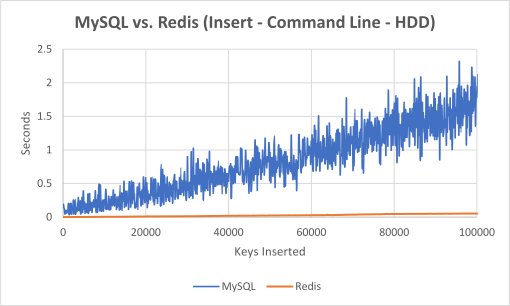
\includegraphics[width=0.5\textwidth]{1.svg}
    \includesvg[width=0.5\textwidth]{svg/1}
    \caption{Performance between MySQL and Redis performing insertion on a HDD.}
    \label{fig:mesh1}
\end{figure}
Knowing that Redis performs in memory as opposed to MySQL makes it much, much faster. At 100000 key-value pairs inserted, Redis performs at 0.0518 seconds, whereas MySQL performs at around 2.1234 seconds. While these results aren't surprising, as Redis is 40.9923x faster than MySQL, we can attempt to do better by switching to a Solid-State Drive (SSD).
\begin{figure}[h]
    \centering
    %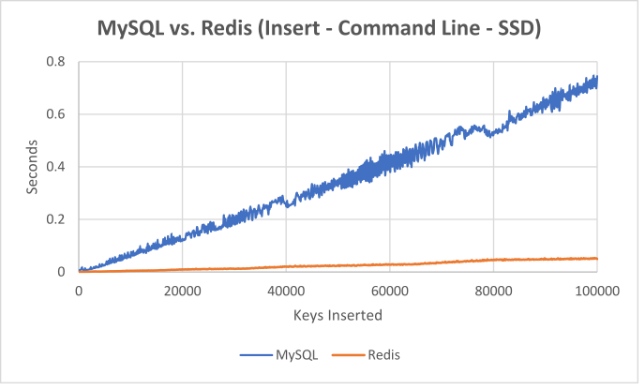
\includegraphics[width=0.5\textwidth]{2.png}
    \includesvg[width=0.5\textwidth]{svg/2}
    \caption{Performance between MySQL and Redis performing insertion on an SSD.}
    \label{fig:mesh1}
\end{figure}
On an SSD the results for Redis's insertion remains the same, as its performance is done in memory. However, MySQL's performance improves drastically. At 100000 keys, it performs at 0.7448 seconds. This is a 2.8509x speedup compared to its HDD test runs, and it is 14.3784x slower than Redis.
\subsubsection{Finds (Reads)}
The test performed here is an find operation of increasingly more keys in a database that already has 100000 keys inserted. The first test consists of a find operation with 100 keys. The second test consists of the same operation but with 200 keys. The test goes on until eventually all 100000 keys are in the query (and inevitably found). \\
For MySQL, the exact query looks like this:
\begin{verbatim}
    MySQL> SELECT * FROM test WHERE t_key
           IN (key1, key2, key3, ...);
\end{verbatim}
For Redis, the exact query look like this:
\begin{verbatim}
    Redis> mget key1 key2 key3 ...
\end{verbatim}
\begin{figure}[h]
    \centering
    %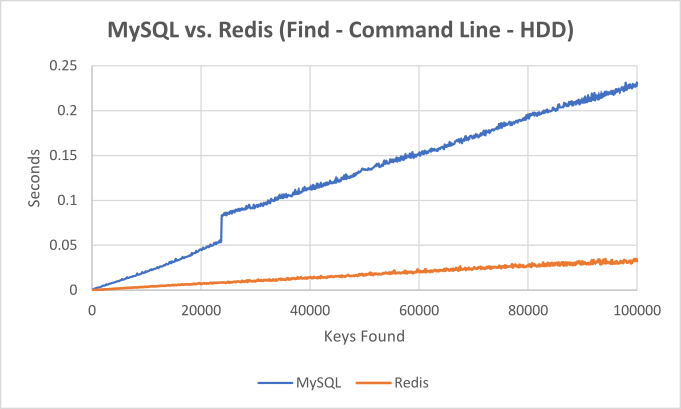
\includegraphics[width=0.5\textwidth]{3.png}
    \includesvg[width=0.5\textwidth]{svg/3}
    \caption{Performance between MySQL and Redis performing finds on a HDD.}
    \label{fig:mesh1}
\end{figure}
Redis's advantage of being in memory, again, allows it to come out ahead of MySQL in terms of reading data. However, there is an interesting spike in performance of MySQL that persists after adding around 23700 or more keys into the query. This performance also holds true in the SSD performance, which leads us to believe that this bottleneck is software-related in the command line application for MySQL. Thankfully, we can actually test if this holds true by running the same tests in Node.JS rather than the C native apps to see if we get different results.
\begin{figure}[h]
    \centering
    %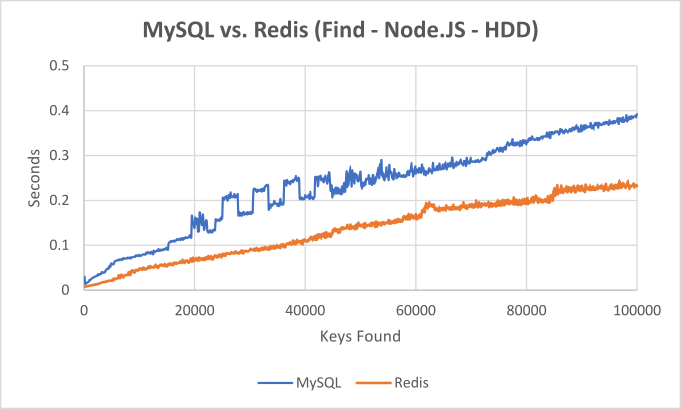
\includegraphics[width=0.5\textwidth]{4.png}
    \includesvg[width=0.5\textwidth]{svg/4}
    \caption{Performance between MySQL and Redis performing finds on a HDD via Node.JS.}
    \label{fig:mesh1}
\end{figure}
Both Redis and MySQL suffer and show different results when using wrapper libraries and packages in Node.JS to communicate with the respective database softwares. However, MySQL has another interesting performance spike within the 20000-50000 key range. This confirms the suspicion of the impact in performance being caused by software.
\subsection{Analysis 2: HDD vs. SSD}
In our previous analysis, we demonstrated some differences between HDD and SSD performance, mainly for the sake of demonstrating MySQL's penalties while inserting on a HDD.
\begin{figure}[h]
    \centering
    %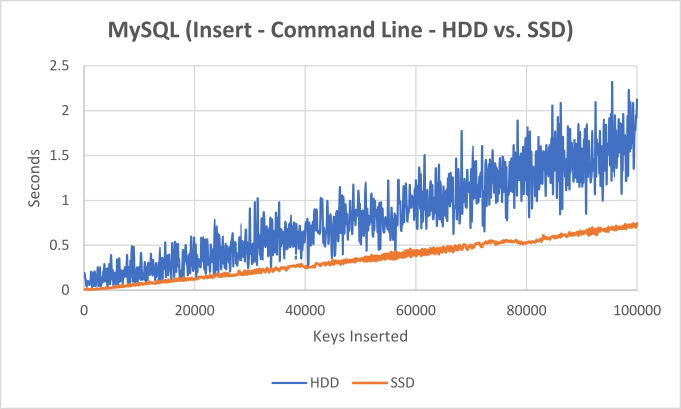
\includegraphics[width=0.5\textwidth]{5.png}
    \includesvg[width=0.5\textwidth]{svg/5}
    \caption{MySQL write performance between HDD and SSD.}
    \label{fig:mesh1}
\end{figure}
This is because, unlike Redis, MySQL relies entirely on I/O with the disk to store the database. This has shown to be a massive bottleneck to MySQL in every test performed comparing it to Redis. However, explicitly comparing HDD to SSD directly yields interesting results on its own. When comparing insertions, the only real cases that had a major impact on performance were the insertions of keys into a MySQL database. The find cases for MySQL, as well as both the insertion and find cases for Redis had minimal impact upon switching a HDD for an SSD. Let's look more into it.
Just like MySQL Insertion, we have other three cases where SSDs have the potential to speed up performance:
\begin{itemize}
    \item MySQL Find
    \item Redis Insertion
    \item Redis Find
\end{itemize}

Let's look into each of them.
\subsubsection{MySQL Find}
\begin{figure}[h]
    \centering
    %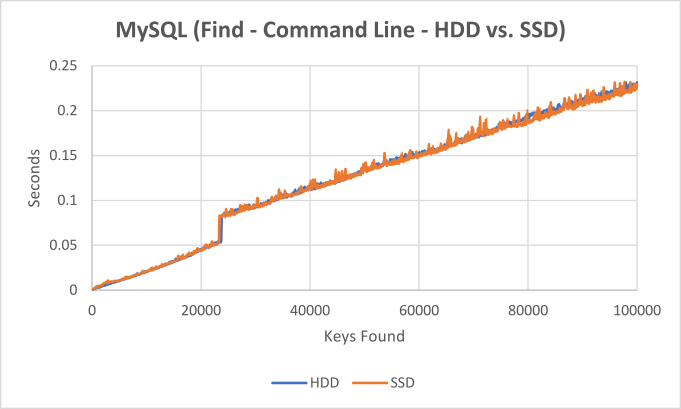
\includegraphics[width=0.5\textwidth]{6.png}
    \includesvg[width=0.5\textwidth]{svg/6}
    \caption{MySQL read performance between HDD and SSD.}
    \label{fig:mesh1}
\end{figure}
This is an interesting case where HDD and SSD appear to have nearly equal performance. Even more interestingly, both the HDD and SSD have the same penalty at around the 23700th key being added into the query. This performance penalty also holds for when Node.JS is used instead, where it also has an interesting spike of duration between the 20000-50000 key range.

Part of the reason for this similar performance is because of how MySQL internally stores its database on the file system. Cleverly, MySQL uses the B-Tree data structure. What makes this special is that, unlike other Binary Search trees (such as AVL and Red-Black), B-Trees are not optimized for being used in memory. They were constructed specifically for storage systems, such as disks. Since the internal structure for MySQL is a B-tree, optimal for disks, the nearly equal performance between both HDD and SSD in the find operation isn't a surprise.
\subsubsection{Redis Insert and Find}
\begin{figure}[h]
    \centering
    %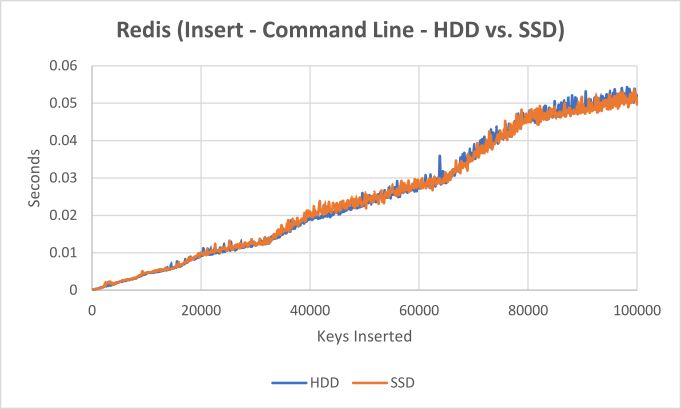
\includegraphics[width=0.5\textwidth]{7.png}
    \includesvg[width=0.5\textwidth]{svg/7}
        \caption{Redis write performance between HDD and SSD.}
    \label{fig:mesh1}
\end{figure}
\begin{figure}[h]
    \centering
    %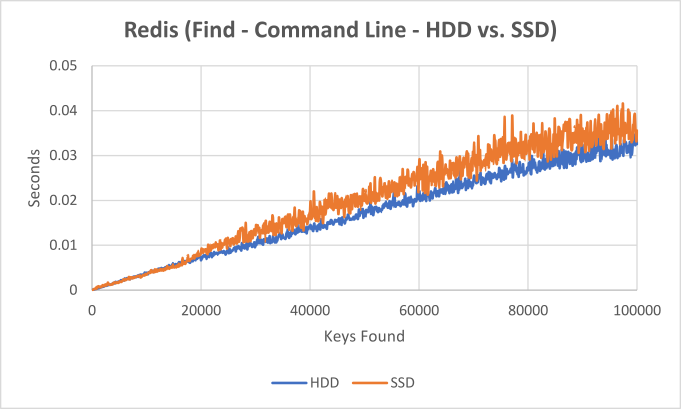
\includegraphics[width=0.5\textwidth]{8.png}
    \includesvg[width=0.5\textwidth]{svg/8}
        \caption{Redis read performance between HDD and SSD.}
    \label{fig:mesh1}
\end{figure}
Redis's performance between a HDD and an SSD is irrelevant, as it is in-memory. Interestingly, the find operation yields a faster time for the HDD benchmark as opposed to the SSD benchmark. However, when run on Node.JS, this penalty goes away. It's possible that this is due to other running software or RAM restrictions on the test bench, rather than between HDD and SSD.
\section{CONCLUSIONS AND FUTURE WORK}

\begin{table}[h]

\caption{Performance of MySQL and Redis on HDD and SSDs with 100000 keys in all queries (in seconds)}
\resizebox{\columnwidth}{!}{%
\begin{tabular}{@{}lllll@{}}
\toprule
\rowcolor[HTML]{DAE8FC} 
                                               & MySQL (HDD)                   & MySQL (SSD)                   & Redis (HDD)                   & Redis (SSD)                   \\ \midrule
Insertion (via Command Line)                   & 2.1234                        & 0.7448                        & 0.0518                        & 0.0497                        \\
\rowcolor[HTML]{DAE8FC} 
{\color[HTML]{000000} Find (via Command Line)} & {\color[HTML]{000000} 0.2314} & {\color[HTML]{000000} 0.2294} & {\color[HTML]{000000} 0.0326} & {\color[HTML]{000000} 0.0356} \\
Insertion (via Node.JS)                        & 2.5508                        & 1.0336                        & 0.2500                        & 0.2370                        \\
\rowcolor[HTML]{DAE8FC} 
Find (via Node.JS)                             & 0.3922                        & 0.3798                        & 0.2314                        & 0.2228                        \\ \bottomrule
\end{tabular}
}
\end{table}
Overall, Redis outperforms MySQL in a simple key-value pair insertion and finding of any size, with MySQL showing a larger performance penalty as the key count grows. When comparing command line to an external wrapper such as with software like Node.JS, performance in every possible field took a hit, regardless of whether the hardware was with an SSD or HDD. This appears to be the case with any number of keys as well, but only for MySQL insertions. The differences between SSD and HDD only mattered for MySQL insertion queries, as no notable difference was found between finding a key via MySQL, as well as Redis in its entirety.

For future work, the authors of this paper would like to extend their study to other key-value storage systems, such as MongoDB, Voldemort, and ArangoDB. Another possible improvement on this study would be to include more test scenarios in the analysis. Several test scenarios that could be useful for the comparison between key-value storage systems 

\section*{ACKNOWLEDGMENTS}

The authors would like to thank Dr. Qing Cao, the professor of COSC560: Advanced Software Systems, for teaching this course and instilling the authors with the tools needed to complete this study. The authors would also like to thank Haoran Niu, the graduate teaching assistant (GTA) for offering advice and guidance on the programming assignments.



%%%%%%%%%%%%%%%%%%%%%%%%%%%%%%%%%%%%%%%%%%%%%%%%%%%%%%%%%%%%%%%%%%%%%%%%%%%%%%%%





\begin{thebibliography}{99}

\bibitem{c1} J. L. Carlson, Redis in action. Shelter Island: Manning, 2013. 
\bibitem{c2} R. Cattell, “Scalable SQL and NoSQL data stores,” ACM SIGMOD Record, vol. 39, no. 4, pp. 12–27, 2011.
\bibitem{c3} R. Elmasri and S. B. Navathe, Fundamentals of database systems. Harlow, Essex: Pearson Education, 2017.
\bibitem{c4}   J. Han, H. E, G. Le, and J. Du, “Survey on NoSQL database,” 2011 6th International Conference on Pervasive Computing and Applications, 2011.

\end{thebibliography}

 


\end{document}
